\newpage
\section{Corpo rigidio}
Descriviamo un corpo rigido come un sistema di punti materiali, le distanze tra
i quali sono constati nel tempo. Punti: 
$$\{\vec{r}_{\alpha=1}^N\} \hspace{15pt} \{m_{\alpha}\}_{\alpha=1}^N \hspace{15pt} d_{\alpha\beta} = ||\vec{r}_{\alpha}(t) - \vec{r}_{\beta}(t)|| = const$$
Le leggi orarie $\vec{r}_{\alpha}(t)$ dei punti del sistema sono vincolate da questa condizione. Detto ciò invece di 3N coordinate indipendenti
ne bastano 6: $\vec{r}_{CM}(3)$ e 3 angoloi. Per il moto planare: $\vec{r}_{CM}(2)$ e 1 angolo.\\\\
Un punto geometrico determinato solo dalle posizioni $\vec{r}_{\alpha}$, come il centro di massa, ha pure distanze constante da tutti gli $\vec{r}_{\alpha}$, quindi $||\vec{r}_{CM} - \vec{r}_{\alpha}(t)|| = const$.
Si dice che tale punto è \textbf{solidale} al corpo rigido.\\\\
Due punti $\vec{r}_1(t), \vec{r}_2(t)$ solidali al C.R. definiscono un \textbf{vettore solidale} $\vec{r}_2(t) - \vec{r}_1(t)$. Conviene introdurre
un sistema di \textbf{assi solidali}, $\hat{x}', \hat{y}', \hat{z}'$ in cui le coordinate dei vettori solidali sono costanti.\\\\
In Geometrica planare (quella che usiano in questo corso):
\begin{figure}[h!]
    \centering
    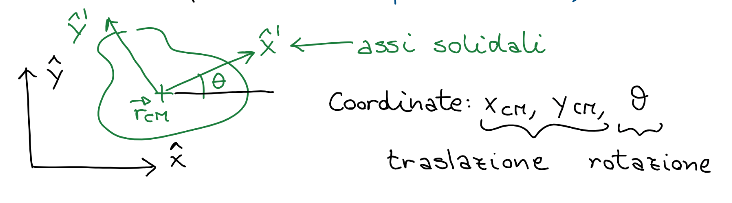
\includegraphics[width=0.65\textwidth]{images/geo-planare.png}
\end{figure}

\hspace{-15pt}Nella Geometria 3D (angoli di eulero):
\begin{figure}[h!]
    \centering
    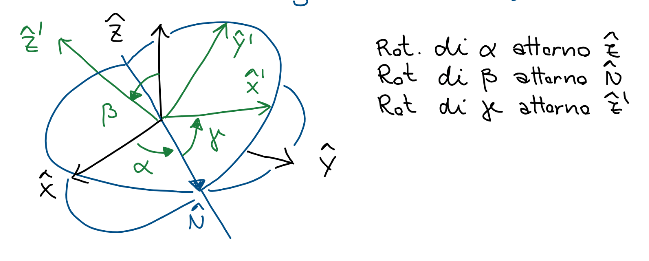
\includegraphics[width=0.55\textwidth]{images/geo-3d.png}
\end{figure}

\subsection{Teorema fondamentale sul moto del corpo rigido}
Il teorema fondamentale sul moto del corpo rigido dice che:
\begin{theorem}
    Ad ogni istante di tempo esiste ed è unico il vettore $\vec{w}(t)$, detto \textbf{vettore velocità angolare}, tale che, dati due punti qualunque $P_1, P_2$
    solidali al C.R.
    $$\dot{\vec{r}}_2(t) = \dot{\vec{r}}_1(t) + \vec{w}(t) \times [\vec{r}_2(t) - \vec{r}_1(t)]$$
    Dove $\vec{w}(t)$ è lo stesso per tutti i punti.
\end{theorem}
\hspace{-15pt}Sviluppiamo la teoria in modo generale, ma in questo corso incontriamo solo i moti planari dove:
$$\vec{r}_{\alpha}(t) = x(t) \hat{x} + y(t)\hat{y} + 0 \cdot \hat{z} \Rightarrow \vec{w}(t) = w(t) \hat{z}$$
\begin{example}
    $t= t_0, \vec{w}(t_0) = w\hat{z}, \dot{\vec{r}}_1(t_0) = v_0\hat{x}$
    $$\dot{\vec{r}}_2(t_0) = v_0\hat{x} + w\hat{z}x[L\hat{x}+ L\hat{y}] = v_0\hat{x} + wL\hat{y} - wL\hat{x} = (v_0 - wL)\hat{x} + wL\hat{y}$$
\end{example}
\begin{observation}
    Il vettore velocità angolare descrive il moto rotatorio del corpo rigido. Vogliamo quindi ottnere una equazione del moto per $\vec{w}(t)$ a partire dalla 2a Eq. 
    cardinale. Svolgiamo i passi necessari in questa lezione e nella prossima.
\end{observation}

\subsection{Momento angolare del corpo rigido}
Il momento angolare del corpo rigido si descrive come:
$$\vec{L}_p = M(\vec{r}_{CM}(t) - \vec{r}_p(t)) \times \dot{\vec{r}}_{CM}(t) + \sum_{\alpha=1}^{N}m_{\alpha}\vec{r}_{\alpha}'(t) \times \dot{\vec{r}}_{\alpha}'(t)$$
Con $M(\vec{r}_{CM}(t) - \vec{r}_p(t)) \times \dot{\vec{r}}_{CM}(t)$ dal CM. Mente $\vec{L}_{CM}(t) \equiv \sum_{\alpha=1}^{N}m_{\alpha}\vec{r}_{\alpha}'(t) \times \dot{\vec{r}}_{\alpha}'(t)$ rispetto al CM
\begin{equation*}
    \begin{split}
        \vec{L}_{CM}(t) & = \sum_{\alpha=1}^{N}[\vec{r}_{\alpha}(t) - \vec{r}_{CM}(t)] \times [\dot{\vec{r}}_{\alpha}(t) - \dot{\vec{r}}_{CM}(t)] = \sum_{\alpha=1}^{N} m_{\alpha}[\vec{r}_{\alpha}(t) - \vec{r}_{CM}(t)] \times [\vec{w}(t) \times [\vec{r}_{\alpha} - \vec{r}_{CM}(t)]]\\
                        & = \sum_{\alpha=1}^{N}m_{\alpha}[\vec{r}_{\alpha}'(t) \cdot \vec{r}_{\alpha}'(t)] \vec{w}(t) - \sum_{\alpha=1}^{N} m_{\alpha} \vec{r}_{\alpha}'(t)[\vec{r}_{\alpha}'(t) \cdot \vec{w}(t)]\\
                        & = \sum_{\alpha=1}^{N}m_{\alpha} 
                        \begin{pmatrix}
                            y_{\alpha}'^2 + z_{\alpha}'^2 & -x'_{\alpha} y'_{\alpha} & -x'_{\alpha}z'_{\alpha} \\
                            -y'_{\alpha}x'_{\alpha} & x_{\alpha}'^2 - z_{\alpha}'^2 & -y'_{\alpha}z'_{\alpha} \\
                            -z'_{\alpha}x'_{\alpha} & -z'_{\alpha}y'_{\alpha} & x_{\alpha}'^2 + y_{\alpha}'^2 
                        \end{pmatrix}
                        \begin{pmatrix}
                            w_{x'}(t)\\
                            w_{y'}(t)\\
                            w_{z'}(t)
                        \end{pmatrix}
    \end{split}
\end{equation*}
Coordinate nella base solidale: costante J.\\\\
La matrice J viene chiamata \textbf{tensore di inerzia} ed è una proprietà del corpo rigido, come la massa o il volume. $[J] = kg \cdot m^2$.
In 3D devo usare una matrice di rotazione con gli angoli di Eulero $w_{x'}, w_{y'}, w_{z'}$. Per moti planari (questo corso) $\vec{L}_p, \vec{L}_{CM}, \vec{w} // \hat{z}$
$$\vec{L}_{CM}(t) = \sum_{\alpha=1}^{N}m_{\alpha}(x_{\alpha}'^2 + y_{\alpha}'^2)w(t) \hat{z}$$
La parte $\sum_{\alpha=1}^{N}m_{\alpha}(x_{\alpha}'^2 + y_{\alpha}'^2)$ è detta $I_{CM}$ che sta per il momento di inerzia assiale. 
\begin{example}
    $I_{CM} = m_1|x_1'|^2 + m_2|x_2'|^2$ (ricordare che per la definizone $m_1x_1' + m_2x_2' = 0$)
\end{example}
\begin{example}
    Momento di inerzia assiale di un cilindro. $V= \pi R^2\cdot h \hspace{10pt}$ densità $\rho = M/V$
    $$I_z = \sum_{\alpha=1}^{N}m_{\alpha}(x_{\alpha}'^2 + y_{\alpha}'^2) = \int dm(x'^2 + y'^2) = \int dx' \int dy' \int_{0}^{h}dz' \cdot \rho(x'^2 + y'^2)$$
    Cambio di variabili nell'integrale per avere estremi più semplici: $x' = r \cdot \cos\Theta, y' = r \cdot \sin\Theta, dx' \cdot dy' = dr \cdot d\Theta \cdot r$
    $$= \int_{0}^{R}dr' \int_{0}^{2\pi}d\Theta' \cdot r'\int_{0}^{n}\cdot \rho \cdot r'^2 = \rho \cdot 2\pi \cdot h \cdot \frac{R^4}{4} = M\frac{1}{\pi R^2 h} \cdot 2\pi \cdot h \cdot \frac{R^4}{4} = \frac{1}{2}MR^2$$
\end{example}